%%%%%%%%%%%%%%%%%%%%%%%%%%%%%%%%%%%%%
% Document properties and packages
%%%%%%%%%%%%%%%%%%%%%%%%%%%%%%%%%%%%%
\documentclass[a3paper,12pt,final]{memoir}
\usepackage{CJKutf8}%中文支持

% misc
\renewcommand{\familydefault}{bch}	% font
\pagestyle{empty}					% no pagenumbering
\setlength{\parindent}{0pt}			% no paragraph indentation
% required packages (add your own)
\usepackage{flowfram}% column layou
\usepackage{marvosym}
\usepackage{textcomp}

\usepackage[top=1cm,left=1cm,right=1cm,bottom=1cm]{geometry}% margins
\usepackage{graphicx}										% figures
\usepackage{hyperref}
\definecolor{linkcolour}{rgb}{0,0.2,0.6}  %蓝色
\hypersetup{colorlinks,breaklinks,urlcolor=linkcolour, linkcolor=linkcolour}										% URLs
\usepackage[usenames,dvipsnames]{xcolor}					% color
\usepackage{multicol}										% columns env.
	\setlength{\multicolsep}{0pt}
\usepackage{paralist}										% compact lists
\usepackage{tikz}

%%%%%%%%%%%%%%%%%%%%%%%%%%%%%%%%%%%%%
% Create column layout
%%%%%%%%%%%%%%%%%%%%%%%%%%%%%%%%%%%%%
% define length commands
\setlength{\vcolumnsep}{\baselineskip}
\setlength{\columnsep}{\vcolumnsep}
%定义主题颜色,可选颜色 Maroon,ForestGreen,DarkOrchid,RoyalBlue,Turquoise,Cyan,etc,更多颜色参考xcolor包的颜色定义
\newcommand{\myThemeColor}{RoyalBlue}
% frame setup (flowfram package)
% left frame
\newflowframe{0.23\textwidth}{\textheight}{0pt}{0pt}[left]
	\newlength{\LeftMainSep}
	\setlength{\LeftMainSep}{0.23\textwidth}
	\addtolength{\LeftMainSep}{1\columnsep}
 
% small static frame for the vertical line
\newstaticframe{1.5pt}{\textheight}{\LeftMainSep}{0pt}
 
% content of the static frame
\begin{staticcontents}{1} %绘制分割线,使用tikz包绘制。如需改变风格线样式,请参考tikz教程,对于新手,不建议修改。
\hfill
\tikz{%
	\draw[loosely dotted,color=\myThemeColor,line width=1.5pt,yshift=0]
	(0,0) -- (0,\textheight);}%
\hfill\mbox{}
\end{staticcontents}
 
% right frame
\addtolength{\LeftMainSep}{1.5pt}
\addtolength{\LeftMainSep}{1\columnsep}
\newflowframe{0.7\textwidth}{\textheight}{\LeftMainSep}{0pt}[main01]


%%%%%%%%%%%%%%%%%%%%%%%%%%%%%%%%%%%%%
% define macros (for convience)
%%%%%%%%%%%%%%%%%%%%%%%%%%%%%%%%%%%%%
\newcommand{\Sep}{\vspace{1em}}
\newcommand{\SmallSep}{\vspace{0.9em}}

\newenvironment{AboutMe}
	{\ignorespaces\textbf{\color{\myThemeColor} About me}}
	{\Sep\ignorespacesafterend}
%定义section	
\newcommand{\CVSection}[1]
	{\Large\textbf{#1}\par
	\vspace{0.2cm}\normalsize\normalfont}

\newcommand{\CVItem}[1]
	{\textbf{\color{\myThemeColor} #1}}


%%%%%%%%%%%%%%%%%%%%%%%%%%%%%%%%%%%%%
% Begin document
%%%%%%%%%%%%%%%%%%%%%%%%%%%%%%%%%%%%%
\begin{document}

\begin{CJK*}{UTF8}{gbsn}%选择字体,黑体
% Left frame 左边内容在此定义
%%%%%%%%%%%%%%%%%%%%
\begin{figure}
	\hfill
	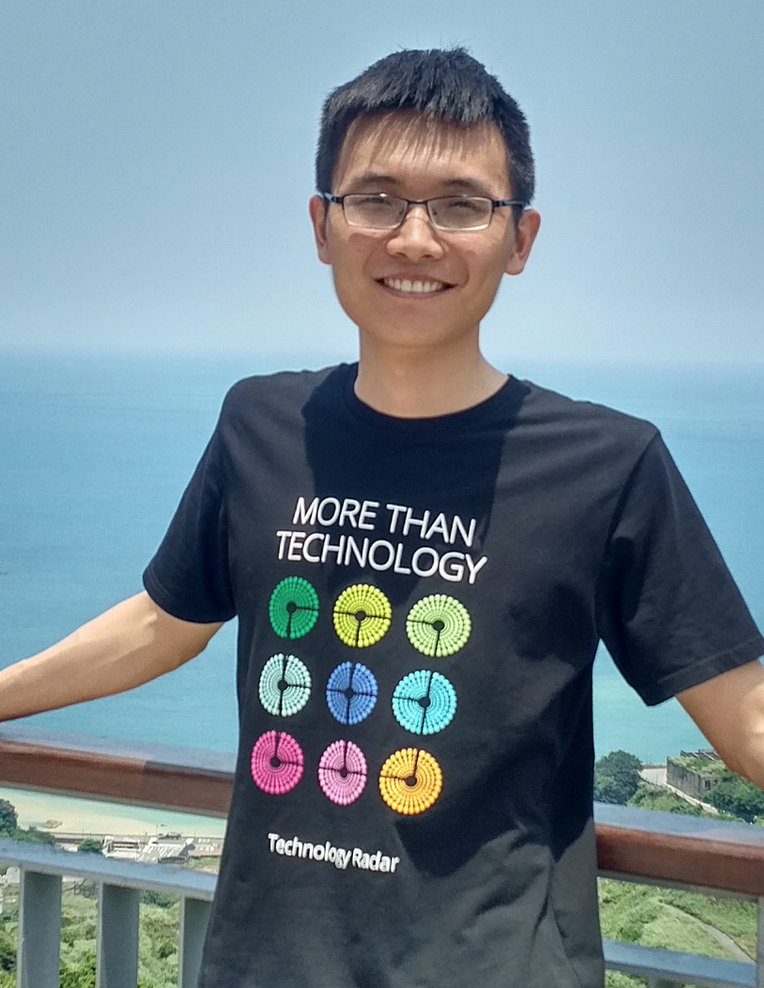
\includegraphics[width=0.7\columnwidth]{photo}
	\vspace{-7cm}
\end{figure}
\begin{flushright}\footnotesize
.\\
\vskip 6cm
\raggedright
\CVItem{{\large Personal Info:}}\\
email:\\
	\href{mailto:clin@thoughtworks.com}{clin@thoughtworks.com}  \\
	website:\\
	\href{http://linchen2chris.github.io/}{linchen2chris.github.io} \\
	phone:\\ 13540394019	
  
	\CVItem{{\large Language:}}\\
  \SmallSep
	\textit{\textbf{Mandarin}:native \\\textbf{English}:fluent\\}
	
  \vskip 1cm
  \CVItem{{\large Education:}}\\
  \SmallSep
	\textit{\textbf{Computer Science Master}\\
    Sichuan University\\
    \textbf{Public Management Bachlor}\\
    Sichuan University\\}

	%% \SmallSep
	%% \textit{能够在Android和WP平台上编写简单的Apps,熟练使用\LaTeX 和LINUX}
	
	%% \CVItem{{\large 爱好:}}\\
	%% \textit{长跑,旅游,摄影,健身,吉他}
	%% \SmallSep
\end{flushright}\normalsize
\framebreak


% Right frame 右边内容在此定义
%%%%%%%%%%%%%%%%%%%%
\Huge\bfseries {\color{\myThemeColor} Lin~~Chen}\\
\normalsize\normalfont

% Education
% \CVSection{教育背景}
% \hrule
% \SmallSep
% \CVItem{2011 - 2014\hfill\textsc{四川大学}}\\
% \textit{-计算机科学与技术专业硕士}\\
% \\
% \CVItem{2007 - 2011\hfill\textsc{四川大学}}\\
% \textit{-公共管理学院本科}\\

% Skills
\CVSection{Skills}
\hrule
\SmallSep
\CVItem{Frontend:}\\
\textit{$\bullet$ react, react-native, typescript, etc} \\
\\
\CVItem{Backend:}\\
\textit{$\bullet$ spring boot/cloud, nodejs, ruby on rails, etc } \\
\\
\CVItem{Devops:}\\
\textit{$\bullet$ AWS, Terraform, Docker, K8s, Service Mesh, etc }\\

\CVItem{other:}\\
\textit{$\bullet$ CI/CD, Agile, Scrum, TDD, etc }\\
\\

% Experience
\CVSection{Experience}
\hrule
\SmallSep
\CVItem{2016.10 - Now \hfill Thoughtworks}\\
\textit{$\bullet$ Senior Consultant, Tech Lead} \\
\textit{$\bullet$ Project 1:Singapore goverment website maintaince(2021.9-2022.2)} \\
\textit{$\bullet$ Project Details: We build the app on react and spring cloud and deploy it on AWS. We are using ECS, lambda, ses, sqs, etc}\\


\textit{$\bullet$ Project 2:Offshore real estate company data platform(2021.2-2021.9)} \\
\textit{$\bullet$ Project Details: We build data pipeline on airflow which will extract and clean data from AWS dynamodb and Salesforce, then push the data to GCP bigquery data marketplace. It mainly use AWS lambda, SQS, SNS, kinesis, GCP bigquery}\\


\textit{$\bullet$ Project 3:Low Code platform(2020.9-2021.2)}\\
\textit{$\bullet$ Project Details: \\\textbf{Frontend:}~react~ \\
  \textbf{Backend:}~spring boot~ }\\


\textit{$\bullet$ Project 4:Employee platform(2020.1-2020.9)} \\
\textit{$\bullet$ Project Details: \\\textbf{Frontend:}~react~ \\
  \textbf{Backend:}~nodejs~ \\
  \textbf{Devops:} We choose as many as possible cloud service to build our app, like stepFunction, Lambda, cloudformation, SES, SQS, SNS, Azure ADFS. Our own frontend and backend services deployed on our K8s platform}\\


\textit{$\bullet$ Project 5: Singapore smart nation app(2018.8-2020.1)} \\
\textit{$\bullet$ Project Details: \\\textbf{Frontend:}~react+react native~; \\
  \textbf{Backend:}~we use Nodejs build micro services~, and Elastic Search for storage and search。\\
  \textbf{Devops:} AWS ELK, ECS, etc. Also choose terraform to do IaC~} \\


\textit{$\bullet$ Project 6:online insurance and bank(2016.10-2018.8)} \\
\textit{$\bullet$ Project Details: \\\textbf{Frontend}~react, redux, babel, webpack2, eslint, prettier.
  We achive 95\%+ test coverage.
  We use sonarQube to scan code.
  We use CSS-module to achive css modular.
  We build mock server on mountbank to isolate frontend and backend development.
  We use storybook to build react component rapidly.
  We extract a shared npm modules and public to internal registry for different projects.
  We use protrator to achieve End2End testing.
  \textbf{Backend} spring boot for microservice architecture, we build bff (Backend for Fontend) for every frontend. We use axway to achieve api gateway. We introduce correlationID to track api logs in all services. we use dozer to transfer data models.we choose pact to achive contract testing.
  B{Database}: PostgreSQL, we use h2 for development
  \textbf{Devops:} AWS, Jenkins for CI/CD, we use blue-green deployment } \\

\CVItem{2015.10 - 2016.10 \hfill one start-up company}\\
\textit{$\bullet$ Role: Full stack Dev} \\
\textit{$\bullet$ Project: Hospital manage system} \\
\textit{$\bullet$ Project Details: nodejs, mongodb, react, redux} \\
\\
\CVItem{2014.07 - 2015.10 \hfill Cinet}\\
\textit{$\bullet$ Role: Backend Dev} \\
\textit{$\bullet$ Project: Telecom Billing System} \\
\textit{$\bullet$ Project Details: we use C/C++ as main language, we login Unix mainframe, using vim, make, gcc to develop apps} \\
% CAMPU
%% \CVSection{专业经历}
%% \hrule
%% \SmallSep
%% \CVItem{2012.04 - 2013.03, 大学生创新项目(IPP)\hfill\emph{研究员}}\\
%% \textit{$\bullet$ 主导参加IPP项目,研究并可视化激光等离子体在真空环境下的聚焦点。} 
%% \\
%% \CVItem{2013.05 - 2013.09, 大陆台湾能源合作\hfill\emph{研究专员}}\\
%% \textit{$\bullet$ 调研大陆能源供给和消费情况,相关资料提供给台湾学者使用,促进两岸科学交流} 
%% \\
%% \CVItem{2013.02 - 2013.10, 奥迪绿色能源竞赛\hfill\emph{团队领导}}\\
%% \textit{$\bullet$ 领头参加绿色能源竞赛,我们的作品是“智能绿色候车公交站台”,并获一等奖}
%% \\
%% \CVItem{2012.06 - 2012.09, 社会实践\hfill\emph{团队领导}}\\
%% \textit{$\bullet$ 组织16个人的社会实践团队,深入甘肃会宁,为一个公益福利网站调查并收集贫困家庭信息,该项目获上海市社会实践优秀项目} 

% HONORS & SCHOLARSHIPS
%% \CVSection{个人荣誉}
%% \hrule
%% \SmallSep
%% 	\begin{tabular}{l|l}
%% 		$\Rightarrow$ 2014.10&\textit{法国大使馆杰出人才奖学金}\footnotesize\\
%% 		$\Rightarrow$ 2013.10&\textit{奥迪绿色能源竞赛一等奖}\\
%% 		$\Rightarrow$ 2012.12&\textit{晨兴企业奖学金}\\
%% 		$\Rightarrow$ 2012.10&\textit{连续三年获得上海交大优秀学生奖学金}\\
%% 		$\Rightarrow$ 2011.04&\textit{上海市社会实践优秀项目}\footnotesize\\
%% 	\end{tabular}

%%%%%%%%%%%%%%%%%%%%%%%%%%%%%%%%%%%%%
% End document
%%%%%%%%%%%%%%%%%%%%%%%%%%%%%%%%%%%%%
\end{CJK*}
\end{document}
